\documentclass[nooutcomes,noauthor,handout,hints]{ximera}

\graphicspath{  
{./}
{./whoAreYou/}
{./drawingWithTheTurtle/}
{./bisectionMethod/}
{./circles/}
{./anglesAndRightTriangles/}
{./lawOfSines/}
{./lawOfCosines/}
{./plotter/}
{./staircases/}
{./pitch/}
{./qualityControl/}
{./symmetry/}
{./nGonBlock/}
}


%% page layout
\usepackage[cm,headings]{fullpage}
\raggedright
\setlength\headheight{13.6pt}


%% fonts
\usepackage{euler}

\usepackage{FiraMono}
\renewcommand\familydefault{\ttdefault} 
\usepackage[defaultmathsizes]{mathastext}
\usepackage[htt]{hyphenat}

\usepackage[T1]{fontenc}
\usepackage[scaled=1]{FiraSans}

%\usepackage{wedn}
\usepackage{pbsi} %% Answer font


\usepackage{cancel} %% strike through in pitch/pitch.tex


%% \usepackage{ulem} %% 
%% \renewcommand{\ULthickness}{2pt}% changes underline thickness

\tikzset{>=stealth}

\usepackage{adjustbox}

\setcounter{titlenumber}{-1}

%% journal style
\makeatletter
\newcommand\journalstyle{%
  \def\activitystyle{activity-chapter}
  \def\maketitle{%
    \addtocounter{titlenumber}{1}%
                {\flushleft\small\sffamily\bfseries\@pretitle\par\vspace{-1.5em}}%
                {\flushleft\LARGE\sffamily\bfseries\thetitlenumber\hspace{1em}\@title \par }%
                {\vskip .6em\noindent\textit\theabstract\setcounter{question}{0}\setcounter{sectiontitlenumber}{0}}%
                    \par\vspace{2em}
                    \phantomsection\addcontentsline{toc}{section}{\thetitlenumber\hspace{1em}\textbf{\@title}}%
                     }}
\makeatother



%% thm like environments
\let\question\relax
\let\endquestion\relax

\newtheoremstyle{QuestionStyle}{\topsep}{\topsep}%%% space between body and thm
		{}                      %%% Thm body font
		{}                              %%% Indent amount (empty = no indent)
		{\bfseries}            %%% Thm head font
		{)}                              %%% Punctuation after thm head
		{ }                           %%% Space after thm head
		{\thmnumber{#2}\thmnote{ \bfseries(#3)}}%%% Thm head spec
\theoremstyle{QuestionStyle}
\newtheorem{question}{}



\let\freeResponse\relax
\let\endfreeResponse\relax

%% \newtheoremstyle{ResponseStyle}{\topsep}{\topsep}%%% space between body and thm
%% 		{\wedn\bfseries}                      %%% Thm body font
%% 		{}                              %%% Indent amount (empty = no indent)
%% 		{\wedn\bfseries}            %%% Thm head font
%% 		{}                              %%% Punctuation after thm head
%% 		{3ex}                           %%% Space after thm head
%% 		{\underline{\underline{\thmname{#1}}}}%%% Thm head spec
%% \theoremstyle{ResponseStyle}

\usepackage[tikz]{mdframed}
\mdfdefinestyle{ResponseStyle}{leftmargin=1cm,linecolor=black,roundcorner=5pt,
, font=\bsifamily,}%font=\wedn\bfseries\upshape,}


\ifhandout
\NewEnviron{freeResponse}{}
\else
%\newtheorem{freeResponse}{Response:}
\newenvironment{freeResponse}{\begin{mdframed}[style=ResponseStyle]}{\end{mdframed}}
\fi



%% attempting to automate outcomes.

%% \newwrite\outcomefile
%%   \immediate\openout\outcomefile=\jobname.oc
%% \renewcommand{\outcome}[1]{\edef\theoutcomes{\theoutcomes #1~}%
%% \immediate\write\outcomefile{\unexpanded{\outcome}{#1}}}

%% \newcommand{\outcomelist}{\begin{itemize}\theoutcomes\end{itemize}}

%% \NewEnviron{listOutcomes}{\small\sffamily
%% After answering the following questions, students should be able to:
%% \begin{itemize}
%% \BODY
%% \end{itemize}
%% }
\usepackage[tikz]{mdframed}
\mdfdefinestyle{OutcomeStyle}{leftmargin=2cm,rightmargin=2cm,linecolor=black,roundcorner=5pt,
, font=\small\sffamily,}%font=\wedn\bfseries\upshape,}
\newenvironment{listOutcomes}{\begin{mdframed}[style=OutcomeStyle]After answering the following questions, students should be able to:\begin{itemize}}{\end{itemize}\end{mdframed}}



%% my commands

\newcommand{\snap}{{\bfseries\itshape\textsf{Snap!}}}
\newcommand{\flavor}{\link[\snap]{https://snap.berkeley.edu/}}
\newcommand{\mooculus}{\textsf{\textbf{MOOC}\textnormal{\textsf{ULUS}}}}


\usepackage{tkz-euclide}
\tikzstyle geometryDiagrams=[rounded corners=.5pt,ultra thick,color=black]
\colorlet{penColor}{black} % Color of a curve in a plot



\ifhandout\newcommand{\mynewpage}{\newpage}\else\newcommand{\mynewpage}{}\fi

\title{Formulas galore}

\author{Bart Snapp}

\begin{document}
\begin{abstract}
  Let's think about formulas.
\end{abstract}
\maketitle


\begin{listOutcomes}
\item Apply formulas to compute the surface areas and volumes of
  solids.
\item Acknowledge that even with a formula, difficult work still needs
  to be done.
\item Identify answers that are incorrect by an order of magnitude or
  more.
\item Use basic number sense to find a reasonable estimate for the
  value of an expression.
\item Estimate surface area and volume up to an order of magnitude.
\item Evaluate estimates as either too large or too small.
\end{listOutcomes}


Here are a bunch of formulas I found on the INTERNET at this site
\begin{center}
  \textit{https://sites.google.com/site/standardbasicengineering/home/useful-formula-for-finding-area-volume-of-solid-figures}
\end{center}
\begin{center}
  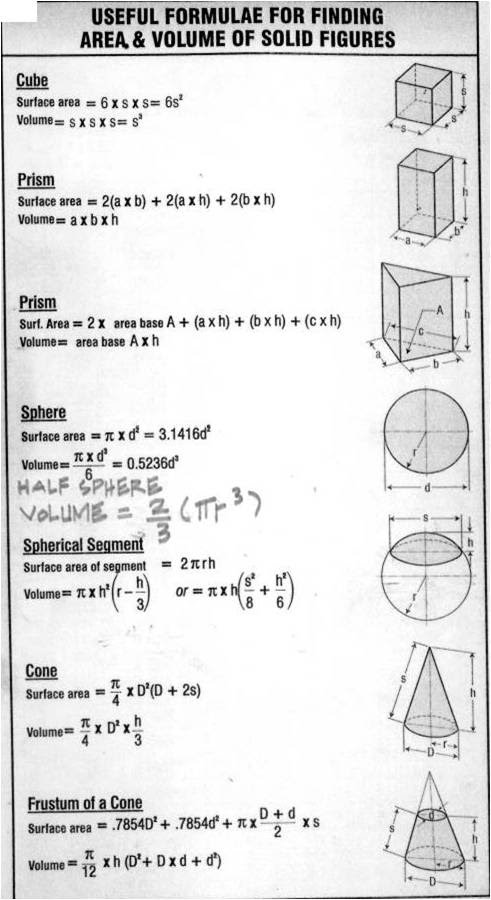
\includegraphics[width=.3\textwidth]{photoFormula1.jpg} \qquad 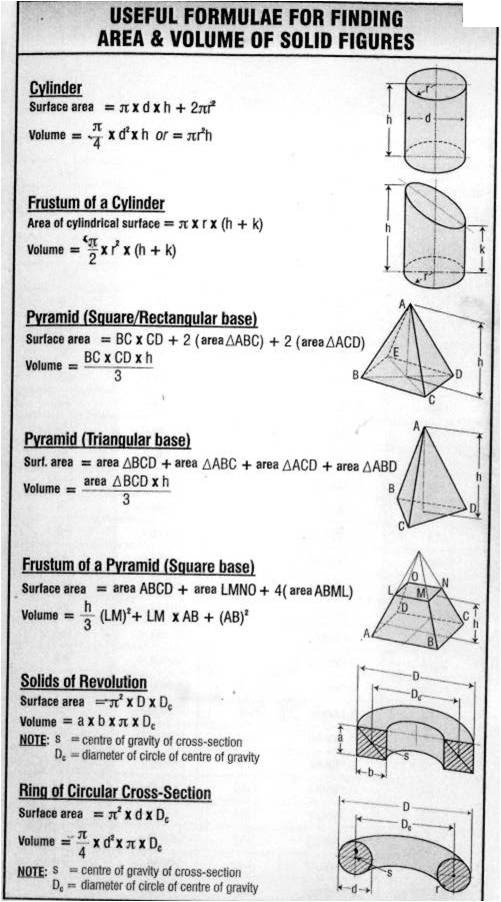
\includegraphics[width=.3\textwidth]{photoFormula2.jpg}
\end{center}

Below, let's think about some questions. 


\mynewpage





\begin{question}
  Consider the \link[\textit{Ericsson Globe}]{https://en.wikipedia.org/wiki/Ericsson_Globe}:
   \begin{center}
    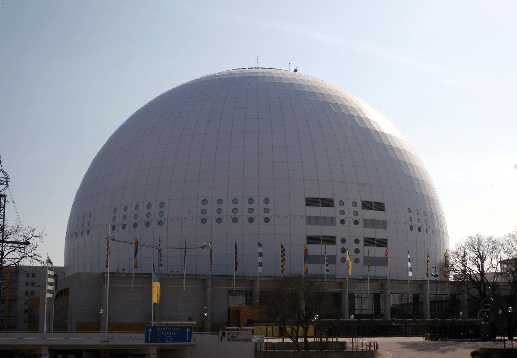
\includegraphics[width=.4\textwidth]{dome.png} %https://www.researchgate.net/figure/Example-of-a-hemispherical-dome-in-modern-civil-engineering-Stockholm-Globe-Arena-by_fig2_308655043
   \end{center}
   Assuming that this building has a diameter of $110$ meters and a
   height of $85$ meters.
   \begin{enumerate}
   \item \label{FG1:1} Use the formulas above to find the surface area
     and the volume of the \textit{Ericsson Globe}.
   \item Estimate the values above by finding the surface area and
     volume of:
     \begin{enumerate}
     \item A box with dimensions $100\times 100 \times 80$.
     \item A box with dimensions $100\times 80 \times 80$.
     \end{enumerate}
   Note: While these answers are NOT EQUAL to your answers from
   part \ref{FG1:1}, these answers \textbf{HAVE THE SAME NUMBER OF
     DIGITS} as your answers from part \ref{FG1:1}.
   \end{enumerate}
   \begin{freeResponse}
     \begin{enumerate}
     \item Using the formulas above I found:
       \[
       SA = 2\pi 55\cdot 85 \approx 29374 \text{ square meters}
       \]
       and
       \[
       V = \pi85^2 \left(55-\frac{85}{3}\right)\approx  605280 \text{ cubic meters}.
       \]
     \item We have two computations.
       \begin{enumerate}
       \item For a box that is  $100\times 100 \times 80$, I find
         \[
         SA = 2(100\cdot 100 + 100\cdot 80 + 100\cdot 80) = 52000 
         \]
         and
         \[
         V = 100\cdot 100\cdot 80 =  800000 
         \]
       \item For a box that is  $100\times 80 \times 80$, I find
         \[
         SA = 2(100\cdot 80 + 80\cdot 80 + 100\cdot 80) = 44800
         \]
         and
         \[
         V = 100\cdot 80\cdot 80 = 640000
         \] 
       \end{enumerate}
       Yup, these answers have the same number of digits as our answers from the first part.       
     \end{enumerate}
   \end{freeResponse}
\end{question}
\mynewpage

\begin{question}
  Consider the \link[\textit{Luxor Las Vegas}]{https://en.wikipedia.org/wiki/Luxor_Las_Vegas}:
  \begin{center}
    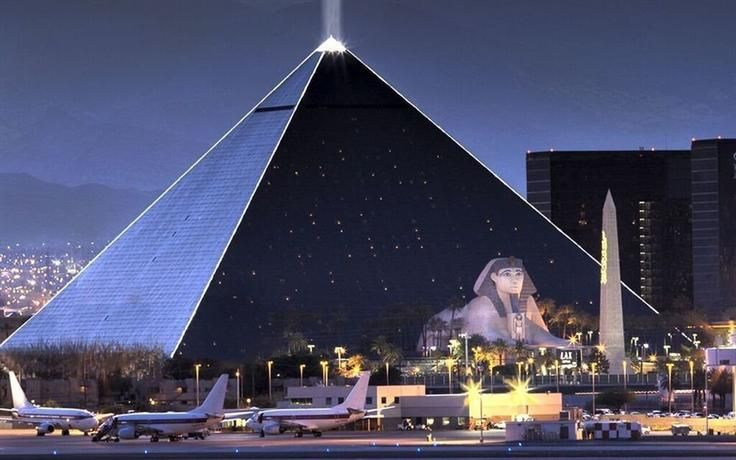
\includegraphics[width=.4\textwidth]{pyramid.jpg} 
  \end{center}
 Assuming that the (square) base of this building has a side length of
 $646$ feet and that the pyramid is $350$ feet tall,
  \begin{enumerate}
  \item Which is EASIER to compute:
    \begin{itemize}
    \item the surface area (including the bottom!) OR
    \item the volume
    \end{itemize}
    of the \textit{Luxor Las Vegas}? EXPLAIN WHY one computation is
    HARDER, and compute the EASIER one.
  \item You ask four friends what the surface area of the
    \textit{Luxor Las Vegas} is. They give you four wrong answers, but
    you love them anyway, because they are your friends. Here are
    their answers:
    \begin{enumerate}
    \item $1500$ square feet
    \item $15000$ square feet
    \item $150000$ square feet
    \item $1500000$ square feet
    \end{enumerate}
    Which answer above is \textbf{closest} to the correct answer? EXPLAIN your reasoning.
  \end{enumerate}
  \begin{freeResponse}
    \begin{enumerate}
      \item The volume is MUCH EASIER to compute than the surface
        area. To compute the surface area, you have to compute the
        area of each face of the pyramid, this requires GEOMETRY.

        The volume is
        \[
        V = \frac{646\cdot 646\cdot 350}{3} \approx = 48686867 \text{ cubic feet}.
        \]
      \item Answer $(iii)$ is correct, here's how I know. The pyramid
        has a base, and four more sides. The biggest the surface area could be is
        \[
        646\cdot 646+ 4\cdot 85\cdot 323 = 869516.
        \]
        But honestly it is even easier:
        \[
        (\text{3-digit number}) \cdot (\text{3-digit number}) + 4\cdot
        (\text{3-digit number}) = (\text{6-digit number}).
        \]
    \end{enumerate}
  \end{freeResponse}
\end{question}
\mynewpage


\begin{question}
  Let's put this together. Estimating a value by knowing the number
  of digits that the answer has, is called \textbf{estimating up to an
    order of magnitude}, because then you know the range of the
  answer.
  \begin{enumerate}
  \item EXPLAIN why 
    \[
    (\text{$m$-digit number}) + (\text{$n$-digit number}) =
    \begin{cases}
      (\text{$\max(m,n)$-digit number}) & \text{or}\\
      (\text{$(1+\max(m,n))$-digit number}),
    \end{cases}
    \]
    and why
    \[
    (\text{$m$-digit number}) \cdot (\text{$n$-digit number}) = \begin{cases}
      (\text{$(m+n)$-digit number}) & \text{or}\\
      (\text{$(m+n-1)$-digit number}).
    \end{cases}
    \]
    \begin{hint}
    Note, every whole number can be written as the product of a number
    between zero and one and a power of ten. For example $253 = .253\cdot 10^3$.
  \end{hint}
  \item Using ideas from this activity, explain how to estimate the
    volume (in cubic feet) and surface area (in square feet) of the \link[Tower at Geisel
      Library]{https://en.wikipedia.org/wiki/Geisel_Library} up to an
    order of magnitude.

  \begin{center}
    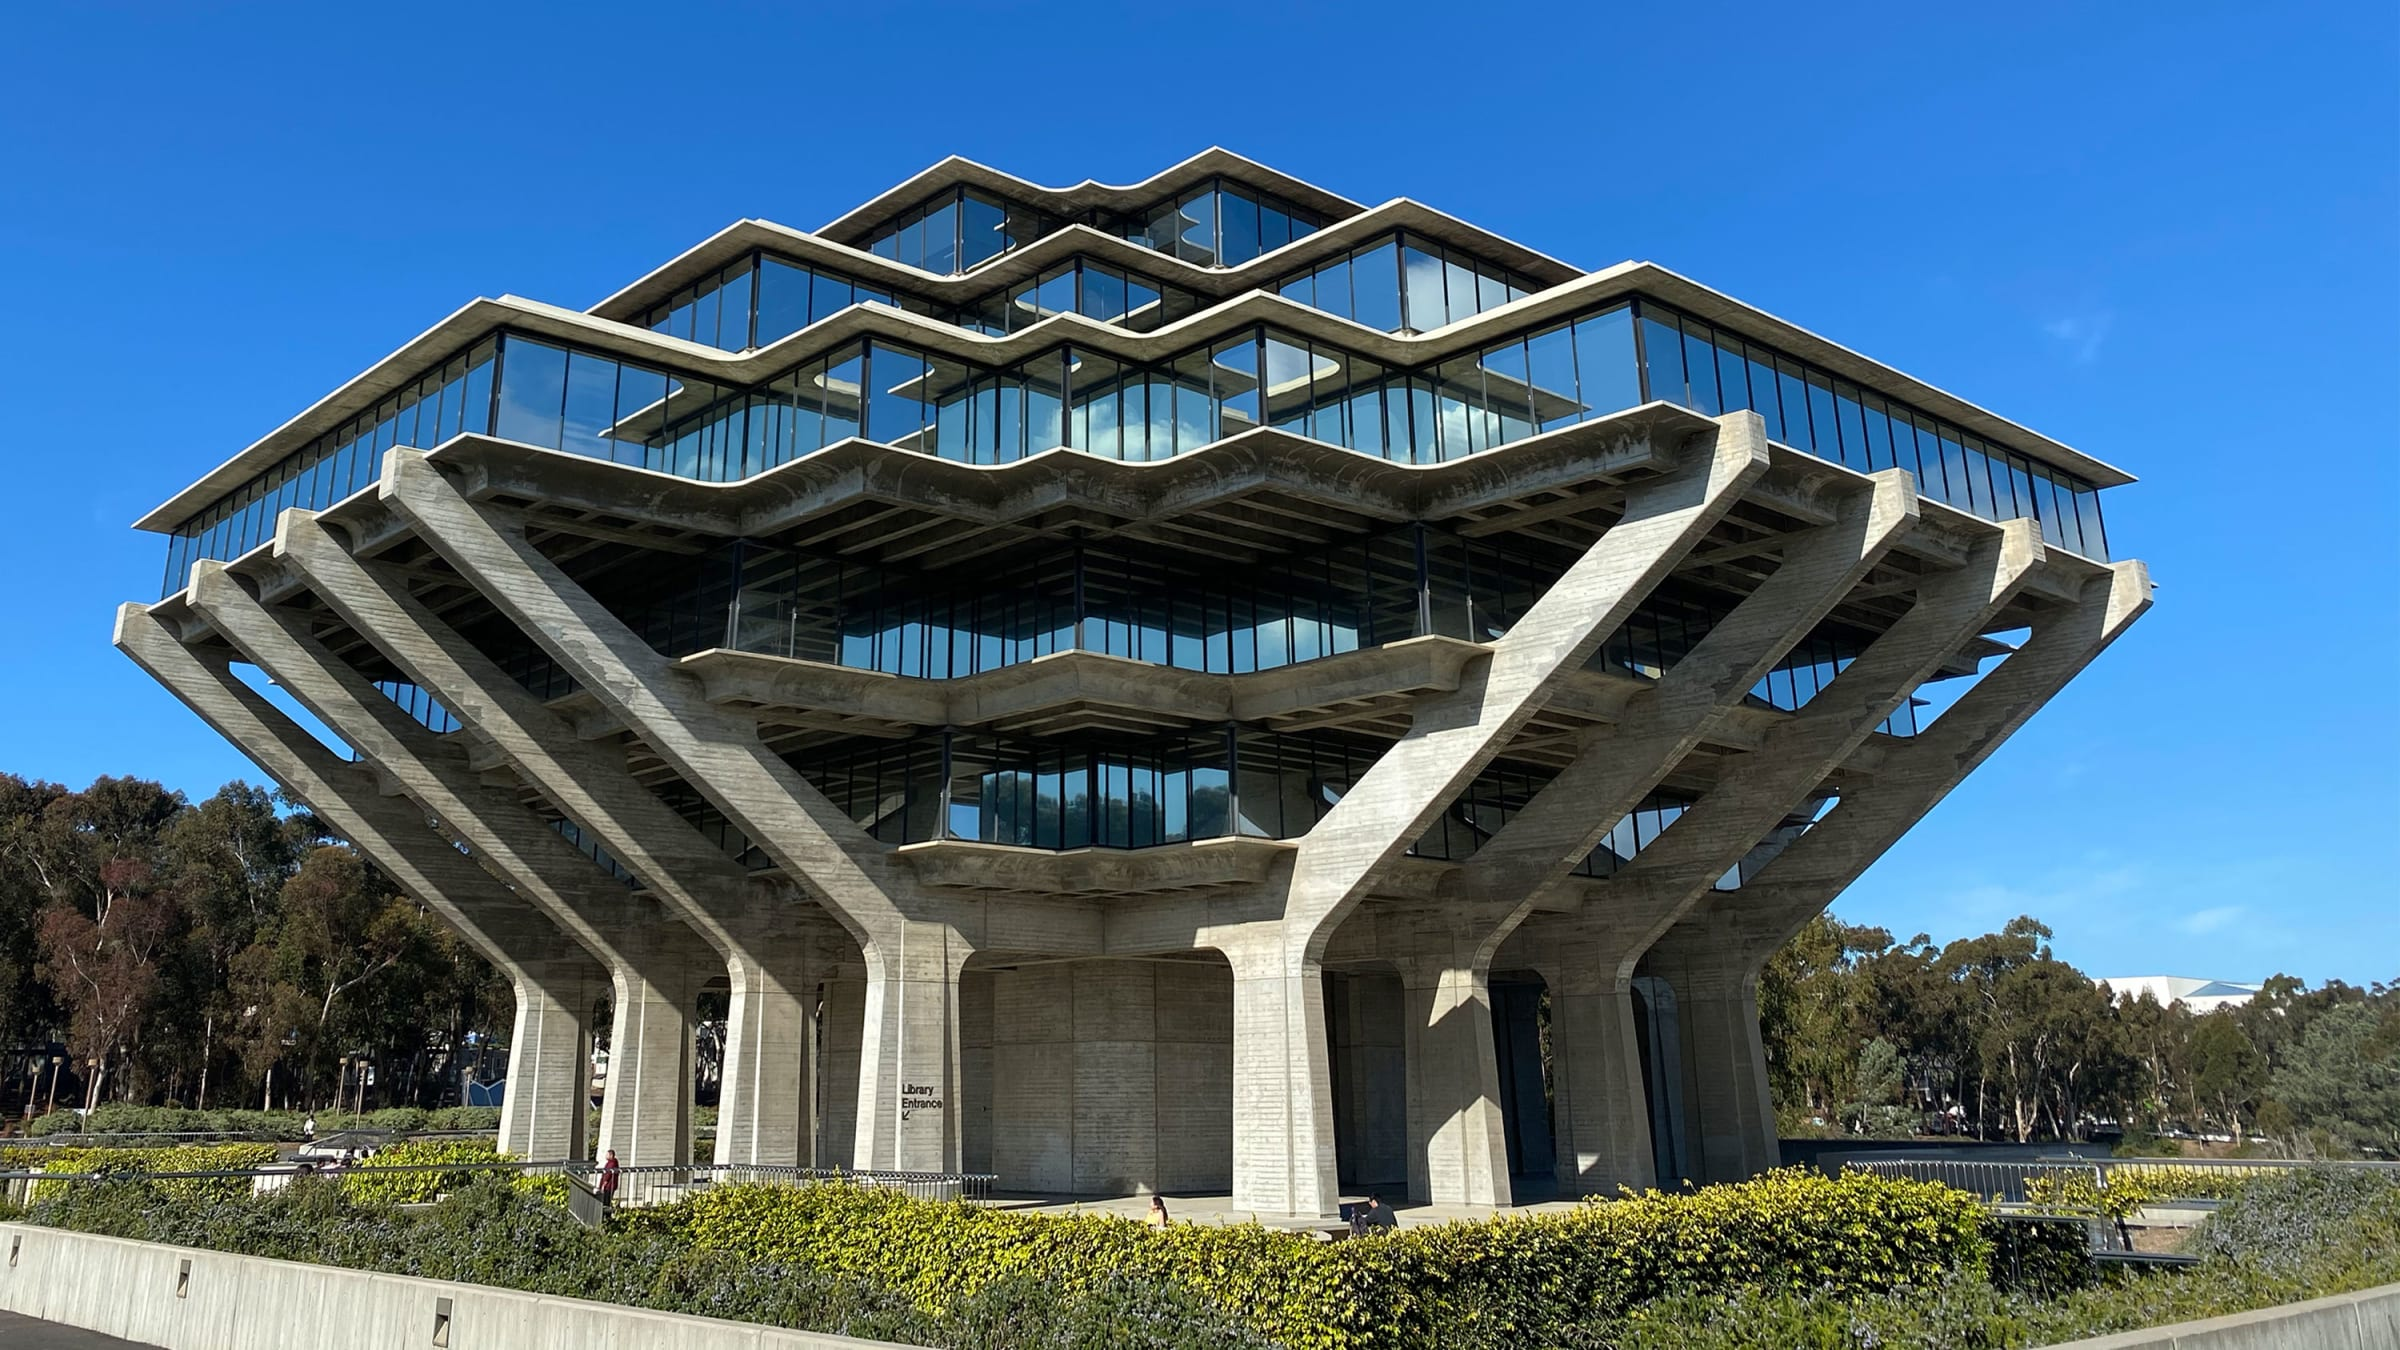
\includegraphics[width=.4\textwidth]{geisel.jpg} 
  \end{center}

    EXPLAIN your reasoning and EXPLAIN if you
    think your estimates are \textbf{too large} or \textbf{too small}
    in each case.
  \end{enumerate}
  
  \begin{freeResponse}
    \begin{enumerate}
    \item So the first statement is true, because if you write our
      numbers as the product of a number between zero and one
      and a power of ten:
      \[
      \underbrace{a\cdot 10^m}_{\text{$m$-digit number}} + \underbrace{b\cdot 10^n}_{\text{$n$-digit number}}
      \]
      where $a$ and $b$ are both between $0$ and $1$, will be a
      $\max(m,n)$-digit number, unless $m=n$ and $a+b>1$, in which case it will be a $(1+\max(m,n))$-digit number.

      For the second statement, if you write our numbers as the
      product of a number between zero and one and a power of ten:
      \[
      \underbrace{a\cdot 10^m}_{\text{$m$-digit number}} \cdot \underbrace{b\cdot 10^n}_{\text{$n$-digit number}} = ab\cdot 10^{m+n}
      \]
      and this is a $(m+n)$-digit number unless $a\cdot b<0.1$, in which
      case it will be a $(m+n-1)$-digit number.
    \item From the Wikipedia page, we see that the tower has a height
      of $110$ feet and a diameter of $200$ feet. Since the tower is so lumpy, I'll estimate the volume as
      \[
      V = 110\cdot 110\cdot 110 = 1331000 \text{ cubic feet}.
      \]
      I believe this estimate is TOO LARGE.

      For the surface area I'll estimate
      \[
      SA = 6(200\cdot 200) = 240000\text{ square feet}.
      \]
      I believe this estimate is TOO SMALL, since the building is so very
      lumpy.
    \end{enumerate}
  \end{freeResponse}
\end{question}
\end{document}
